\section{Fondamenti fisici e matematici dei sistemi a due stati}
Il modello del sistema a due stati è un approccio allo studio di un sistema estremamente utile: da un lato è di facile analisi e dall'altro è molto versatile.\\ 
Un sistema di questo tipo (come particelle con spin $\frac{1}{2}$ o un quibit) è caratterizzato dalla proprietà di poter assumere due soli stati differenti. Questa proprietà si traduce matematicamente nella richiesta di avere uno spazio degli stati a due dimensioni. Sulla base di questa sola richiesta si può costruire un formalismo operatoriale noto come \emph{formalismo di Pauli}.

\subsection{Formalismo di Pauli}
Come si è detto inizialmente, lo spazio degli stati è uno spazio $2-D$ complesso. Questa struttura comporta che su di essi potranno agire una serie di operatori lineari che formano uno spazio vettoriale di dimensione $4$ su campo complesso. Infatti in uno spazio finito dimensionale $2D$ questi operatori sono matrici di $4$ elementi complessi.\\Sia $\hat{A}$ un qualsivoglia operatore, allora sarà scomponibile nella combinazione lineare di $4$ operatori:
\begin{equation*}
    \hat{A}=a_m\hat{I}+a_1\hat{\sigma}_1+a_2\hat{\sigma}_2+a_3\hat{\sigma}_3=a_m\hat{I}+\underline{a}\cdot\hat{\underline{\sigma}},
\end{equation*} 
dove $\underline{a}=(a_1,a_2,a_3)$ e $\hat{\underline{\sigma}}=(\hat{\sigma}_1,\hat{\sigma}_2,\hat{\sigma}_3)$.\\
La scelta di $\hat{\underline{\sigma}}$ è arbitraria ma può essere fatta in maniera tale da garantire alcune proprietà particolari. In primo luogo si richiede che tutte le sue componenti siano autoaggiunte ($\hat{\underline{\sigma}}^*=\hat{\underline{\sigma}}$), così facendo $\hat{A}$ è autoaggiunto se tutti i coefficienti numerici sono reali.\\
In secondo luogo si richiede che valga:
\begin{equation*}
    (\underline{a}\cdot\hat{\underline{\sigma}})(\underline{b}\cdot\hat{\underline{\sigma}})=\underline{a}\cdot\underline{b}\hat{I}+i\underline{a}\times \underline{b}\cdot \hat{\underline{\sigma}}.
\end{equation*}
Questa richiesta è impartita da tre ragioni:
\begin{itemize}
    \item il prodotto $(\underline{a}\cdot\hat{\underline{\sigma}})(\underline{b}\cdot\hat{\underline{\sigma}})$ è a sua volta un operatore e quindi deve essere espresso come combinazione lineare dei $4$ operatori utilizzati per $\hat{A}$,
    \item l'uso di prodotti scalari e vettoriali garantisce la linearità rispetto ai due fattori,
    \item l'unità immaginaria è necessaria affinché valga $[(\underline{a}\cdot\hat{\underline{\sigma}})(\underline{b}\cdot\hat{\underline{\sigma}})]^*=(\bar{\underline{b}}\cdot\hat{\underline{\sigma}})(\bar{\underline{a}}\cdot\hat{\underline{\sigma}})$.
\end{itemize}
\begin{definition}[Operatore di Pauli]
    Sia $\hat{\underline{\sigma}}=(\hat{\sigma}_1,\hat{\sigma}_2,\hat{\sigma}_3)$, tale che $\hat{\underline{\sigma}}^*=\hat{\underline{\sigma}}$, allora se valgono
    \begin{flalign*}
        &[\underline{a}\cdot\hat{\underline{\sigma}},\underline{b}\cdot\hat{\underline{\sigma}}]=2i\underline{a}\times \underline{b}\cdot \hat{\underline{\sigma}},\\&
        (\underline{a}\cdot\hat{\underline{\sigma}})(\underline{b}\cdot\hat{\underline{\sigma}})+(\underline{b}\cdot\hat{\underline{\sigma}})(\underline{a}\cdot\hat{\underline{\sigma}})=2\underline{a}\cdot\underline{b}\hat{I},
    \end{flalign*}
    questo è un \emph{operatore di Pauli}.
\end{definition}
\begin{remark}
    Si osservi che queste due richieste sono del tutto analoghe a quella precedente (infatti esplicitando il commutatore e sommando queste due si ottiene la condizione iniziale).
\end{remark}
\subsection{Problema agli autovalori}
Si vuole studiare il problema agli auto valori dell'operatore autoaggiunto $\hat{A}$:
\begin{equation*}
    \hat{A}=a_m\hat{I}+a\underline{n}\cdot\hat{\underline{\sigma}},
\end{equation*}
dove $\underline{n}$ è un versore di componenti reali tale che $a\underline{n}=\underline{a}$.\\
Siccome ogni ket è autoket dell'identità il problema considerato si riduce a quello di trovare lo spettro di $\underline{n}\cdot\hat{\underline{\sigma}}$. Gli operatori di Pauli garantiscono la seguente proprietà.
\begin{proposition}
    Lo spettro di $\underline{n}\cdot\hat{\underline{\sigma}}$ è $\{-1,+1\}$.
\end{proposition}
\begin{proof}
    Gli autoket di $\underline{n}\cdot\hat{\underline{\sigma}}$ formano una base ortonormale $\{\ket{\underline{n},+1},\ket{\underline{n},-1}\}$ (poiché questo è autoaggiunto). Il problema agli autovalori è quindi:
    \begin{equation*}
        \underline{n}\cdot\hat{\underline{\sigma}}\ket{\underline{n},\pm1}=\ket{\underline{n},\pm1}\lambda_{\pm}.
    \end{equation*}
    Il Teorema spettrale invece garantisce la seguente rappresentazione di $(\underline{n}\cdot\hat{\underline{\sigma}})^2$:
    \begin{flalign*}
        (\underline{n}\cdot\hat{\underline{\sigma}})^2=\ket{\underline{n},+1}\lambda_{+}^2\bra{\underline{n},+1}+\ket{\underline{n},-1}\lambda_{-}^2\bra{\underline{n},-1},
    \end{flalign*}
    questa quantità può essere anche calcolata dalle proprietà richieste per un operatore di Pauli:
    \begin{equation*}
        (\underline{n}\cdot\hat{\underline{\sigma}})^2=(\underline{n}\cdot\underline{n})\hat{I}+i(\underline{n}\times\underline{n})\cdot\hat{\underline{\sigma}}=\hat{I}.
    \end{equation*}
    Da quest'ultima si ha che $\lambda_{\pm}^2=1$.
    Si osservi che non è possibile che $\lambda_{+}=\lambda_{-}$, altrimenti l'operatore $\underline{n}\cdot\hat{\underline{\sigma}}$, dal Teorema spettrale, sarebbe un multiplo dell'identità. Se questo fosse vero allora questo operatore di Pauli commuterebbe con tutti gli altri operatori, cosa non consentita dalla sua definizione.\\
    Si conclude che il suo spettro è $\{-1,+1\}$ (convenzionalmente si fanno coincidere i segni degli autovalori con quelli degli autoket).
\end{proof}
Se ora si applica uno degli autoket di $\underline{n}\cdot\hat{\underline{\sigma}}$ all'operatore $\hat{A}$ si ottiene:
\begin{equation*}
    \hat{A}\ket{\underline{n},\pm1}=[a_m\hat{I}+a\underline{n}\cdot\hat{\underline{\sigma}}]\ket{\underline{n},\pm1}=\ket{\underline{n},\pm1}(a_m\pm a),
\end{equation*}
per cui vale la seguente proposizone.
\begin{proposition}
    Lo spettro di $\hat{A}=a_m\hat{I}+a\underline{n}\cdot\hat{\underline{\sigma}}$ è $\{a_m+a,a_m- a\}$.
\end{proposition}
\subsection{Basi ortonormali per rappresentare operatori}
Si è precedentemente discusso di come sia possibile rappresentare un operatore autoaggiunto tramite la combinazione lineare:
\begin{equation*}
    \hat{A}=a_m\hat{I}+a\underline{n}\cdot\hat{\underline{\sigma}}.
\end{equation*}
Il vettore $\underline{a}=a\underline{n}$ è un vettore di $\mathbb{R}^3$ (affinché sia autoaggiunto $\hat{A}$) e per questo deve poter essere proiettato sulla base canonica.
\begin{definition}[Base ortonormale orientata]
    Si dice \emph{base ortonormale orientata} l'insieme dei versori $\{\underline{e}_1,\underline{e}_3,\underline{e}_3\}$ tali che $\bar{\underline{e}}_i=\underline{e}_1$ e che siano soddisfatte:
    \begin{flalign*}
        &\underline{e}_i\cdot\underline{e}_j=\delta_{ij}\\
        &\underline{e}_i\times\underline{e}_j=\sum_{k=1}^{3}\epsilon_{ijk}\underline{e}_k.
    \end{flalign*}
    ($\epsilon_{ijk}$ è il simbolo di Levi-Civita.)
\end{definition}
Analogamente si può definire un seconda base che risulta molto utile per svariati conti.
\begin{definition}[Base sferica orientata]
    Si dice \emph{base sferica orientata} l'insieme dei vettori $\{\underline{e}_-1,\underline{e}_0,\underline{e}_1\}$ tali che $\bar{\underline{e}}_\alpha=\underline{e}_{-\alpha}$ e che siano soddisfatte:
    \begin{flalign*}
        &\underline{e}_\alpha\cdot\underline{e}_\beta=2^{|\alpha|}\delta_{-\alpha\beta}\\
        &\underline{e}_\alpha\times\underline{e}_\beta=-i\delta_{\alpha0}\beta\underline{e}_\beta+i\delta_{\beta0}\alpha\underline{e}_\alpha-i\delta_{-\alpha\beta}(\alpha-\beta)\underline{e}_0.
    \end{flalign*}
\end{definition}
Queste due basi sono strettamente collegate, nella fattispecie esiste una corrispondenza uno ad uno data dalle seguenti relazioni (per i vettori delle basi e le componenti di un vettore $\underline{a}$):
\begin{flalign*}
    &\underline{e}_0=\underline{e}_3,\quad\underline{e}_{\pm1}=\underline{e}_1\pm i\underline{e}_2,\quad \underline{e}_1=\frac{\underline{e}_{+1}+\underline{e}_{-1}}{2},\quad \underline{e}_{2}=\frac{\underline{e}_{+1}-\underline{e}_{-1}}{2i},\\
    &a_0=a_3,\quad a_{\pm1}=a_1\pm ia_2,\quad a_1=\frac{a_{+1}+a_{-1}}{2},\quad a_{2}=\frac{a_{+1}-a_{-1}}{2i}.
\end{flalign*}
Le medesime relazioni si applicano agli operatori di Pauli:
\begin{equation*}
    \hat\sigma_0=\hat\sigma_3,\quad \hat\sigma_{\pm1}=\hat\sigma_1\pm i\hat\sigma_2,\quad \hat\sigma_1=\frac{\hat\sigma_{+1}+\hat\sigma_{-1}}{2},\quad \hat\sigma_{2}=\frac{\hat\sigma_{+1}-\hat\sigma_{-1}}{2i}.
\end{equation*}
\subsection{Matrici di Pauli}
Si vuole ora esplicitare la forma degli operatori di Pauli come matrici. Si comincierà dalla base ortogonale, le relazioni tra una base e l'altra consentiranno di determinare tali matrici anche per quella sferica. Si seguirà un argomento non del tutto rigoroso ma efficacie.\\

Nella base ortonormale orientata è possibile scegliere una base ortonormale di autoket dell'operatore $\hat\sigma_3$. Per quanto dimostrato lo spettro questo operatore è $\{-1,+1\}$, per cui: 
\begin{equation*}
    \hat\sigma_3\ket{\underline{e}_3,\pm1}=\ket{\underline{e}_3,\pm1}(\pm1).
\end{equation*}
Il teorema spettrale consente di ottenere la rappresentazione matriciale di questo operatore:
\begin{equation*}
    \hat\sigma_3=\ket{\underline{e}_3,+1}\bra{\underline{e}_3,+1}-\ket{\underline{e}_3,-1}\bra{\underline{e}_3,-1}\Longrightarrow\boxed{\sigma_3=
    \begin{pmatrix}
        1&0\\
        0&-1\\
    \end{pmatrix}}\ .
\end{equation*}

Si consideri ora una matrice $M$ autoaggiunta, la si vuole decomporre nelle matrici di Pauli. Studiando l'aggiunta $M*$ (nel caso delle matrici queste devono essere anche trasposte):
\begin{equation*}
    \begin{pmatrix}
        m_1&m_2\\
        m_3&m_4
    \end{pmatrix}=\begin{pmatrix}
        m_1^*&m_3^*\\
        m_2^*&m_4^*
    \end{pmatrix}\quad\Longrightarrow\quad m_1,m_4\in\mathbb{R},\ m_3=m_2^*
\end{equation*}
La base su cui si scomporrà $M$ è formata dalla matrice identità e le tre matrici di Pauli. Per far questo si ridefiniscano i termini della matrice  in maniera tale da ottenere un termine dato da $\hat{I}$ e un termine dato da $\hat\sigma_3$:
\begin{equation*}
    m_1=a+b,\qquad m_4=a-b,\qquad m_3=c+id, \qquad m_2=c-id.
\end{equation*}
La matrice $M$ si scompone nei quattro termini desiderati:
\begin{equation*}
    M=\begin{pmatrix}
        a+b&c+id\\
        c-id&a-b
    \end{pmatrix}=a\begin{pmatrix}
        1&0\\
        0&1
    \end{pmatrix}+b\begin{pmatrix}
        1&0\\
        0&-1
    \end{pmatrix}+c\begin{pmatrix}
        0&1\\
        1&0
    \end{pmatrix}
    +d\begin{pmatrix}
        0&i\\
        -i&0
    \end{pmatrix}
\end{equation*}
In coordinate ortonormali orientate si ha quindi:
\begin{equation*}
    \boxed{
        \sigma_1=\begin{pmatrix}
            0&1\\
            1&0
        \end{pmatrix},\qquad
        \sigma_1=\begin{pmatrix}
            0&i\\
            -i&0
        \end{pmatrix},\qquad
        \sigma_3=\begin{pmatrix}
            1&0\\
            0&-1
        \end{pmatrix}
    }\ .
\end{equation*}
Facendo uso delle trasformazioni degli operatori di Pauli, in coordinate sferiche si ha:
\begin{equation*}
    \boxed{
        \sigma_0=\begin{pmatrix}
            1&0\\
            0&-1
        \end{pmatrix},\qquad
        \sigma_{+1}=\begin{pmatrix}
            0&2\\
            0&0
        \end{pmatrix},\qquad
        \sigma_{-1}=\begin{pmatrix}
            0&0\\
            2&0
        \end{pmatrix}
    }\ .
\end{equation*}
\subsection{Esponenziale di Pauli}
\begin{theorem}
    Sia $\underline{n}$ un versore, allora vale la seguente uguaglianza
    \begin{equation*}
        \exp\bigg(i\frac{\vartheta}{2}\underline{n}\cdot\hat{\underline{\sigma}}\bigg)=\cos\bigg(\frac{\vartheta}{2}\bigg)\hat{I}+i\sin\bigg(\frac{\vartheta}{2}\bigg)\underline{n}\cdot\hat{\underline{\sigma}}.
    \end{equation*}
\end{theorem}
\begin{proof}
    Si consideri gli operatori $\ket{\underline{n},\pm1}\bra{\underline{n},\pm1}$ sommando e sottraendo opportuni termini (così che si stia sommando una quantità nulla) si ottiene:
    \begin{equation*}
        \ket{\underline{n},\pm1}\bra{\underline{n},\pm1}=\frac{1}{2}[\ket{\underline{n},+1}\bra{\underline{n},+1}+\ket{\underline{n},-1}\bra{\underline{n},-1}\pm(\ket{\underline{n},+1}\bra{\underline{n},+1}-\ket{\underline{n},-1}\bra{\underline{n},-1})].
    \end{equation*}
    Riconoscendo che, per il Teorema spettrale, $\ket{\underline{n},+1}\bra{\underline{n},+1}+\ket{\underline{n},-1}\bra{\underline{n},-1}=\hat{I}$ e $\ket{\underline{n},+1}\bra{\underline{n},+1}-\ket{\underline{n},-1}\bra{\underline{n},-1}=\underline{n}\cdot\hat{\underline{\sigma}}$, si ottiene:
    \begin{equation*}
        \ket{\underline{n},\pm1}\bra{\underline{n},\pm1}=\frac{\hat{I}\pm\hat{\underline{\sigma}}}{2}.
    \end{equation*}
    Utilizzando il Teorema spettrale per l'operatore $\exp\bigg(i\frac{\vartheta}{2}\underline{n}\cdot\hat{\underline{\sigma}}\bigg)$ si ha:
    \begin{flalign*}
        \exp\bigg(i\frac{\vartheta}{2}\underline{n}\cdot\hat{\underline{\sigma}}\bigg)&=\ket{\underline{n},+1}\exp\bigg(\frac{\vartheta}{2}\bigg)\bra{\underline{n},+1}+\ket{\underline{n},-1}\exp\bigg(-\frac{\vartheta}{2}\bigg)\bra{\underline{n},-1}\\
        &=\exp\bigg(\frac{\vartheta}{2}\bigg)\frac{\hat{I}+\hat{\underline{\sigma}}}{2}+\exp\bigg(-\frac{\vartheta}{2}\bigg)\frac{\hat{I}-\hat{\underline{\sigma}}}{2}=\cos\bigg(\frac{\vartheta}{2}\bigg)\hat{I}+i\sin\bigg(\frac{\vartheta}{2}\bigg)\underline{n}\cdot\hat{\underline{\sigma}}.
    \end{flalign*}
\end{proof}
\subsection{Rotazioni degli autospazi}
Si considerino due operatori $\underline{u}\cdot\hat{\underline{\sigma}}$ e $\underline{v}\cdot\hat{\underline{\sigma}}$ ($\underline{u},\ \underline{v}$ versori), ognuno con autoket, rispettivamente, $ \ket{\underline{u},\pm1}$ e $ \ket{\underline{v},\pm1}$. Si desidera trovare una relazione tra gli autoket di un operatore e l'altro.\\
Si osservi che i due operatori in questione possono essere interpretati come sempre il medesimo operatore ruotato prima nella direzione del primo versore e poi in quella del secondo. In virtù di questa analogia si procede nel seguente modo.
\begin{definition}
    Dati gli operatori $\underline{u}\cdot\hat{\underline{\sigma}}$ e $\underline{v}\cdot\hat{\underline{\sigma}}$ ($\underline{u},\ \underline{v}$ versori) si definiscono l'angolo di rotazione $\vartheta$ e il versore $\underline{k}$ dalle:
    \begin{equation*}
        \cos(\vartheta)=\underline{v}\cdot\underline{u},\qquad\underline{k}=\frac{\underline{v}\times\underline{u}}{|\underline{v}\times\underline{u}|}.
    \end{equation*}\label{def:Angolo Versore Rotazione Operatori}
\end{definition}
Il formalismo di Pauli fornisce il seguente risultato per tale rotazione:
\begin{theorem}
    Dati gli operatori $\underline{u}\cdot\hat{\underline{\sigma}}$ e $\underline{v}\cdot\hat{\underline{\sigma}}$ ($\underline{u},\ \underline{v}$ versori), l'angolo di rotazione $\vartheta$ e il versore $\underline{k}$, tra questi operatori vale la seguente relazione:
    \begin{equation*}
        \exp\bigg(i\frac{\vartheta}{2}\underline{k}\cdot\hat{\underline{\sigma}}\bigg)\underline{u}\cdot\hat{\underline{\sigma}}\exp\bigg(-i\frac{\vartheta}{2}\underline{k}\cdot\hat{\underline{\sigma}}\bigg)=\underline{v}\cdot\hat{\underline{\sigma}}.
    \end{equation*}
    Mentre, tra i loro autoket vale:
    \begin{equation*}
        \ket{\underline{v},\pm1}=\exp\bigg(i\frac{\vartheta}{2}\underline{k}\cdot\hat{\underline{\sigma}}\bigg)\ket{\underline{u},\pm1}.
    \end{equation*}
\end{theorem}
\begin{proof}
    Utilizzando l'esponenziale di Pauli si ottiene:
    \begin{flalign*}
        &\exp\bigg(i\frac{\vartheta}{2}\underline{k}\cdot\hat{\underline{\sigma}}\bigg)\underline{u}\cdot\hat{\underline{\sigma}}\exp\bigg(-i\frac{\vartheta}{2}\underline{k}\cdot\hat{\underline{\sigma}}\bigg)\\
        &=\bigg[\cos\bigg(\frac{\vartheta}{2}\bigg)\hat{I}+i\sin\bigg(\frac{\vartheta}{2}\bigg)\underline{k}\cdot\hat{\underline{\sigma}}\bigg]\underline{u}\cdot\hat{\underline{\sigma}}\bigg[\cos\bigg(\frac{\vartheta}{2}\bigg)\hat{I}-i\sin\bigg(\frac{\vartheta}{2}\bigg)\underline{k}\cdot\hat{\underline{\sigma}}\bigg]\\
        &=\cos^2\bigg(\frac{\vartheta}{2}\bigg)\underline{u}\cdot\hat{\underline{\sigma}}+\sin^2\bigg(\frac{\vartheta}{2}\bigg)(\underline{k}\cdot\hat{\underline{\sigma}})(\underline{u}\cdot\hat{\underline{\sigma}})(\underline{k}\cdot\hat{\underline{\sigma}})+\\ &\qquad\qquad\qquad\qquad+i\cos\bigg(\frac{\vartheta}{2}\bigg)\sin\bigg(\frac{\vartheta}{2}\bigg)[(\underline{k}\cdot\hat{\underline{\sigma}})(\underline{u}\cdot\hat{\underline{\sigma}})-(\underline{u}\cdot\hat{\underline{\sigma}})(\underline{k}\cdot\hat{\underline{\sigma}})].
    \end{flalign*}
    Usando le richieste fatte per definire gli operatori di Pauli
    \begin{equation*}
        (\underline{a}\cdot\hat{\underline{\sigma}})(\underline{b}\cdot\hat{\underline{\sigma}})=\underline{a}\cdot\underline{b}\hat{I}+i\underline{a}\times \underline{b}\cdot \hat{\underline{\sigma}},\qquad [\underline{a}\cdot\hat{\underline{\sigma}},\underline{b}\cdot\hat{\underline{\sigma}}]=2i\underline{a}\times \underline{b}\cdot \hat{\underline{\sigma}},
    \end{equation*}
    e che $\underline{k}\perp\underline{u},\underline{v}$, si ottiene:
    \begin{flalign*}
        (\underline{k}\cdot\hat{\underline{\sigma}})(\underline{u}\cdot\hat{\underline{\sigma}})(\underline{k}\cdot\hat{\underline{\sigma}})&=[\underline{k}\cdot\underline{u}\hat{I}+i\underline{k}\times \underline{u}\cdot \hat{\underline{\sigma}}](\underline{k}\cdot\hat{\underline{\sigma}})=(i\underline{k}\times \underline{u}\cdot \hat{\underline{\sigma}})(\underline{k}\cdot\hat{\underline{\sigma}})\\&=i\underline{k}\times \underline{u}\cdot\underline{k}\hat{I}+i(i\underline{k}\times \underline{u}\times \underline{k})\cdot \hat{\underline{\sigma}}=-(\underline{k}\times \underline{u}\times \underline{k})\cdot \hat{\underline{\sigma}}\\&=-[\underline{u}(\underline{k}\cdot\underline{k})+\underline{k}(\underline{u}\cdot\underline{k})]\cdot\underline{\sigma}=-\underline{u}\cdot\underline{\sigma},
    \end{flalign*}
    e usando che $\underline{k}=\underline{v}\times\underline{u}$ e $\sin{\vartheta}=|\underline{v}\times\underline{u}|$ si ha:
    \begin{flalign*}
        (\underline{k}\cdot\hat{\underline{\sigma}})(\underline{u}\cdot\hat{\underline{\sigma}})-(\underline{u}\cdot\hat{\underline{\sigma}})(\underline{k}\cdot\hat{\underline{\sigma}})&=[\underline{k}\cdot\hat{\underline{\sigma}},\underline{u}\cdot\hat{\underline{\sigma}}]=2i\underline{k}\times\underline{u}\cdot\hat{\underline{\sigma}}=2i\frac{\underline{v}\times\underline{u}\times\underline{u}}{|\underline{v}\times\underline{u}|}\cdot\hat{\underline{\sigma}}\\&=\frac{2i}{\sin{\vartheta}}[(\underline{u}\cdot\underline{v})\underline{u}-\underline{v}]\cdot\hat{\underline{\sigma}}.
    \end{flalign*}
    Infine ricordando le formule trigonometriche 
    \begin{equation*}
        \cos(2x)=\cos^2(x)-\sin^2(x),\qquad\qquad\sin(2x)=2\sin(x)\cos(x),
    \end{equation*}
    e inserendo gli ultimi due risultati nella prima equazione, si ottiene:
    \begin{flalign*}
        &\exp\bigg(i\frac{\vartheta}{2}\underline{k}\cdot\hat{\underline{\sigma}}\bigg)\underline{u}\cdot\hat{\underline{\sigma}}\exp\bigg(-i\frac{\vartheta}{2}\underline{k}\cdot\hat{\underline{\sigma}}\bigg)\\
        &=\cos^2\bigg(\frac{\vartheta}{2}\bigg)\underline{u}\cdot\hat{\underline{\sigma}}-\sin^2\bigg(\frac{\vartheta}{2}\bigg)\underline{u}\cdot\hat{\underline{\sigma}}-2\cos\bigg(\frac{\vartheta}{2}\bigg)\sin\bigg(\frac{\vartheta}{2}\bigg)\frac{1}{\sin{\vartheta}}[(\underline{u}\cdot\underline{v})\underline{u}-\underline{v}]\cdot\hat{\underline{\sigma}}\\&=\cos(\vartheta)\underline{u}\cdot\hat{\underline{\sigma}}-\sin(\vartheta)\frac{1}{\sin{\vartheta}}[(\underline{u}\cdot\underline{v})\underline{u}-\underline{v}]\cdot\hat{\underline{\sigma}}=(\underline{u}\cdot\underline{v})\underline{u}\cdot\hat{\underline{\sigma}}-[(\underline{u}\cdot\underline{v})\underline{u}-\underline{v}]\cdot\hat{\underline{\sigma}}=\underline{v}\cdot\hat{\underline{\sigma}}.
    \end{flalign*}
    La relazione per gli autoket è verificata da un conto diretto:
    \begin{flalign*}
        \underline{v}\cdot\hat{\underline{\sigma}}\ket{\underline{v},\pm1}&= \exp\bigg(i\frac{\vartheta}{2}\underline{k}\cdot\hat{\underline{\sigma}}\bigg)\underline{u}\cdot\hat{\underline{\sigma}}\exp\bigg(-i\frac{\vartheta}{2}\underline{k}\cdot\hat{\underline{\sigma}}\bigg)\ket{\underline{v},\pm1}\\
        &=\exp\bigg(i\frac{\vartheta}{2}\underline{k}\cdot\hat{\underline{\sigma}}\bigg)\underline{u}\cdot\hat{\underline{\sigma}}\exp\bigg(-i\frac{\vartheta}{2}\underline{k}\cdot\hat{\underline{\sigma}}\bigg)\exp\bigg(i\frac{\vartheta}{2}\underline{k}\cdot\hat{\underline{\sigma}}\bigg)\ket{\underline{u},\pm1}\\
        &=\exp\bigg(i\frac{\vartheta}{2}\underline{k}\cdot\hat{\underline{\sigma}}\bigg)\underline{u}\cdot\hat{\underline{\sigma}}\ket{\underline{u},\pm1}=\exp\bigg(i\frac{\vartheta}{2}\underline{k}\cdot\hat{\underline{\sigma}}\bigg)\ket{\underline{u},\pm1}(\pm1)=\ket{\underline{v},\pm1}(\pm1).
    \end{flalign*}
\end{proof}
\begin{example}
    Si vuole esprimere l'autoket $\ket{\underline{n},\pm1}$, dell'operatore $\underline{n}\cdot\hat{\underline{\sigma}}$, in funzione degli autoket $\ket{\underline{e_3},\pm1}$, dell'operatore $\hat{\sigma}_3$.\\

    In primo luogo si determinano:
    \begin{equation*}
        \cos\vartheta=\underline{n}\cdot\underline{e}_3=n_3,\qquad \underline{k}=\frac{\underline{n}\times\underline{e}_3}{|\underline{n}\times\underline{e}_3|}=\frac{n_2\underline{e}_1-n_1\underline{e}_2}{\sqrt{n_1^2+n_2^2}}.
    \end{equation*}
    L'operatore che consente di passare da un autospazio all'altro è quindi dato dall'esponenziale di Pauli:
    \begin{equation*}
        \exp\bigg(i\frac{\vartheta}{2}\underline{n}\cdot\hat{\underline{\sigma}}\bigg)=\cos\bigg(\frac{\vartheta}{2}\bigg)\hat{I}+i\sin\bigg(\frac{\vartheta}{2}\bigg)\underline{n}\cdot\hat{\underline{\sigma}}=\cos\bigg(\frac{\vartheta}{2}\bigg)\hat{I}+i\sin\bigg(\frac{\vartheta}{2}\bigg)\frac{n_2\hat{\sigma}_1-n_1\hat{\sigma}_2}{\sqrt{n_1^2+n_2^2}}
    \end{equation*}
    A questo punto è utile passare alle coordinate sferiche orientate (queste semplificano i conti):
    \begin{flalign*}
        &\underline{e}_0=\underline{e}_3 \qquad\Rightarrow\qquad\cos\vartheta=n_0,\\
        &n_1^2+n_2^2=\bigg(\frac{n_{+1}+n_{-1}}{2}\bigg)^2+\bigg(\frac{n_{+1}-n_{-1}}{2i}\bigg)^2=n_{+1}n_{-1},\\
        &n_2\hat{\sigma}_1-n_1\hat{\sigma}_2=\frac{n_{+1}-n_{-1}}{2i}\frac{\sigma_{+1}+\sigma_{-1}}{2}-\frac{n_{+1}+n_{-1}}{2}\frac{\sigma_{+1}-\sigma_{-1}}{2i}=\frac{i}{2}[n_{-1}\sigma_{+1}-n_{+1}\sigma_{-1}],\\
        &\Rightarrow\qquad\underline{n}\cdot{\hat{\underline{\sigma}}}=i\frac{n_{-1}\sigma_{+1}-n_{+1}\sigma_{-1}}{2\sqrt{n_{+1}n_{-1}}}.
    \end{flalign*}
    Si definisca $\exp{(\pm i\varphi)}=\sqrt{\frac{n_{\pm1}}{n_{\mp1}}}$, così facendo l'esponenziale di Pauli diviene:
    \begin{equation*}
        \exp\bigg(i\frac{\vartheta}{2}\underline{n}\cdot\hat{\underline{\sigma}}\bigg)=\cos\bigg(\frac{\vartheta}{2}\bigg)\hat{I}-\frac{1}{2}\sin\bigg(\frac{\vartheta}{2}\bigg)[\exp(-i\varphi)\hat{\sigma}_{+1}-\exp(i\varphi)\hat{\sigma}_{-1}].
    \end{equation*}
    Dovendo applicare questo operatore ai ket $\ket{n_3,\pm}=\ket{n_0,\pm}$ è opportuno calcolare $\hat{\sigma}_{\pm}$ applicato a questi (siccome appaiono nella sua espressione esplicita). Dalla rappresentazione in coordinate sferiche degli operatori di Pauli si ha:
\begin{flalign*}
    &\hat{\sigma}_{\pm1}\ket{n_0,\pm1}=2\ket{n_0,\pm1}\braket{n_0,\mp1|n_0,\pm}=0,\\
    &\hat{\sigma}_{\pm1}\ket{n_0,\mp1}=2\ket{n_0,\pm1}\braket{n_0,\mp1|n_0,\mp1}=2\ket{n_0,\pm1}.
\end{flalign*}
Si può quindi procedere esplicitando la relazione:
\begin{flalign*}
    \ket{\underline{n},+1}&=\exp\bigg(i\frac{\vartheta}{2}\underline{n}\cdot\hat{\underline{\sigma}}\bigg)\ket{e_0,+1}\\&=\cos\bigg(\frac{\vartheta}{2}\bigg)\hat{I}-\frac{1}{2}\sin\bigg(\frac{\vartheta}{2}\bigg)[\exp(-i\varphi)\hat{\sigma}_{+1}-\exp(i\varphi)\hat{\sigma}_{-1}]\ket{e_0,+1}\\
    \Rightarrow\quad&\boxed{\ket{\underline{n},+1}=\ket{e_0,+1}\cos\bigg(\frac{\vartheta}{2}\bigg)+\ket{e_0,+1}\sin\bigg(\frac{\vartheta}{2}\bigg)\exp(i\varphi)}\ ,\\
    \ket{\underline{n},-1}&=\exp\bigg(i\frac{\vartheta}{2}\underline{n}\cdot\hat{\underline{\sigma}}\bigg)\ket{e_0,-1}\\&=\cos\bigg(\frac{\vartheta}{2}\bigg)\hat{I}-\frac{1}{2}\sin\bigg(\frac{\vartheta}{2}\bigg)[\exp(-i\varphi)\hat{\sigma}_{+1}-\exp(i\varphi)\hat{\sigma}_{-1}]\ket{e_0,-1}\\
    \Rightarrow\quad&\boxed{\ket{\underline{n},-1}=\ket{e_0,-1}\cos\bigg(\frac{\vartheta}{2}\bigg)-\ket{e_0,-1}\sin\bigg(\frac{\vartheta}{2}\bigg)\exp(-i\varphi)}\ .
\end{flalign*}
Dove si ricorda $\cos\vartheta=n_0=n_3$ e $\exp{(\pm i\varphi)}=\sqrt{\frac{n_{\pm1}}{n_{\mp1}}}=\sqrt{\frac{n_1\pm in_2}{n_1\mp in_2}}$.\label{example:nSigma0}
\end{example}
\begin{remark}
    Si osservi che così facendo lo stato $\ket{\underline{n},\pm1}$ è parametrizzato su una sfera.\\ Infatti al variare di $\underline{n}$ varieranno i parametri angolari $\vartheta,\ \varphi$ muovendosi su di una superficie sferica chiamata \emph{sfera di Bloch}.  
\end{remark}
\section{Modellizzare un sistema a due livelli}
Si desidera ora applicare ad un sistema fisico la struttura algebrica descritta nella precedente sezione. Un sistema a soli due stati raramente corrisponde alla realtà fisica ma spesso rappresenta una prima approssimazione del sistema (per esempio supponendo che solo i primi due livelli energetici possano essere occupati).
\subsection{Hamiltoniano a due livelli}
Un sistema a due livelli energetici è quindi caratterizzato da due stati con due energie differenti, rispettivamente $\ket{\pm1}$ e $h_{\pm1}$ ($h_{+1}>h_{-1}$). Si può costruire l'hamiltoniano del sistema sfruttando questa osservazione e il Teorema spettrale:
\begin{flalign*}
    \hat{H}=\ket{+1}h_{+1}\bra{+1}+\ket{-1}h_{-1}\bra{-1}.
\end{flalign*}
Definendo i parametri $h_{m}=\frac{h_{+1}+h_{-1}}{2}$ (energia media) e $\Delta{h}=h_{+1}-h_{-1}$ (separazione dei livelli) l'hamiltoniano può essere riscritta come:
\begin{flalign*}
    \hat{H}&=\ket{+1}\bigg(h_{m}+\frac{\Delta h}{2}\bigg)\bra{+1}+\ket{-1}\bigg(h_{m}-\frac{\Delta h}{2}\bigg)\bra{-1}\\&=h_m\bigg[\ket{+1}\bra{+1}+\ket{-1}\bra{-1}\bigg]+\frac{\Delta h}{2}\bigg[\ket{+1}\bra{+1}-\ket{-1}\bra{-1}\bigg]=h_{m}\hat{I}+\frac{\Delta h}{2}\hat{\sigma}_3.
\end{flalign*}
Si è così mostrato come costruire una corrispondenza diretta tra sistema a due livelli energetici e formalismo di Pauli.
\begin{figure}[H]
    \centering
    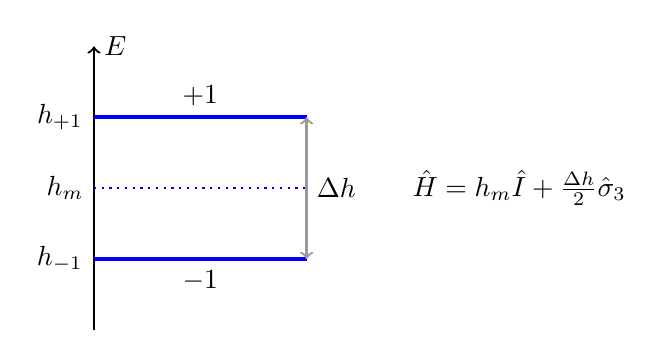
\begin{tikzpicture}[scale=0.9]
        \draw[->,black,thick] (0,-1) -- (0,3)node[anchor=west]{$E$};
        \draw[blue,ultra thick] (0,0)node[anchor=east,black]{$h_{-1}$} --node[anchor=north,black]{$\ket{-1}$} (3,0);
        \draw[blue,ultra thick] (0,2)node[anchor=east,black]{$h_{+1}$}  --node[anchor=south,black]{$\ket{+1}$} (3,2);
        \draw[blue, thick,dotted] (0,1)node[anchor=east,black]{$h_{m}$}  -- (3,1);
        \draw[<->,black!40,thick] (3,0) --node[anchor=west,black]{$\Delta h$} (3,2);
        \node at (6,1) {$\boxed{\hat{H}=h_{m}\hat{I}+\frac{\Delta h}{2}\hat{\sigma}_3}$};
    \end{tikzpicture}
\end{figure}
\subsection{Perturbazioni di un sistema a due livelli}
Spesso e volentieri identificare lo stato di un sistema, seppur a due soli livelli, può essere complesso. In questi casi si può considerare un sistema più semplice, per il quale è facile identificare gli stati del sistema, per esprimere lo stato del sistema reale in funzione di quello più semplice.\\

Si considera quindi un hamiltoniano imperturbato $\hat{H}_0=h_{0,m}\hat{I}+\frac{\Delta h_{0}}{2}\hat{\sigma}_0$\footnote{Si stanno usando le coordinate sferiche orientate.}, che da origine a due autostati $\ket{0,\pm1}$. Una perturbazione del sistema è rappresentata da un operatore autoaggiunto che può quindi essere espresso in funzione degli operatori di Pauli:
\begin{equation*}
    \hat{W}=w_m\hat{I}+\underline{w}\cdot\underline{\hat{\sigma}}\quad\Rightarrow\quad\hat{H}=\hat{H}_0+\hat{W}=(h_{0,m}+w_m)\hat{I}+\bigg(\frac{\Delta h_{0}}{2}\underline{e}_0+\underline{w}\bigg)\cdot\underline{\hat{\sigma}}.
\end{equation*}
Si avranno quindi due autoket di $\hat{H}$ con i loro rispettivi autovalori (determinati dalla teoria degli operatori di Pauli):
\begin{equation*}
    \hat{H}\ket{\pm 1}=\ket{\pm 1}h_{\pm1},\qquad h_{\pm1}=h_{0,m}+w_m\pm\bigg|\frac{\Delta h_{0}}{2}\underline{e}_0+\underline{w}\bigg|.
\end{equation*}
Come si è visto è possibile esprimere questi autoket (e i loro autovalori) in funzione di quelli dell'operatore $\hat{H}$:
\begin{equation*}
    \ket{\pm1}=\ket{0,\pm1}\cos\bigg(\frac{\vartheta}{2}\bigg)\pm\ket{0,\pm1}\sin\bigg(\frac{\vartheta}{2}\bigg)\exp(\pm i\varphi).
\end{equation*}
Per determinare $\vartheta$ e $\varphi$ è necessario identificare prima il versore $\underline{n}$ dell'operatore di Pauli perturbato (in questo modo si possono usare le formule ottenute nell'Esempio \ref{example:nSigma0}):
\begin{equation*}
    \underline{n}=\frac{\frac{\Delta h_{0}}{2}\underline{e}_0+\underline{w}}{\bigg|\frac{\Delta h_{0}}{2}\underline{e}_0+\underline{w}\bigg|} \quad \Rightarrow\quad \cos\vartheta=\underline{n}\cdot\underline{e}_0=\frac{\frac{\Delta h_{0}}{2}+w_0}{\bigg|\frac{\Delta h_{0}}{2}\underline{e}_0+\underline{w}\bigg|},\qquad \exp(\pm i \varphi)=\sqrt{\frac{n_{\pm1}}{n_{\mp1}}}=\sqrt{\frac{w_{\pm1}}{w_{\mp1}}}.
\end{equation*}
Infine definendo $h_{m}=\frac{h_{+1}+h_{-1}}{2}$ (energia media) e $\Delta{h}=h_{+1}-h_{-1}$ (separazione dei livelli) si ha:
\begin{equation*}
    h_m=h_{0,m}+w_m,\qquad\Delta{h}=|\Delta h_0\underline{e}_0+2\underline{w}|.
\end{equation*}
Si osservi che, seppure queste quantità possano sembrare facilmente ricavabili, in particolar modo l'autovalore energetico può essere alquanto complesso da calcolare (per via della presenza del modulo vettoriale).
\begin{figure}[H]
    \centering
    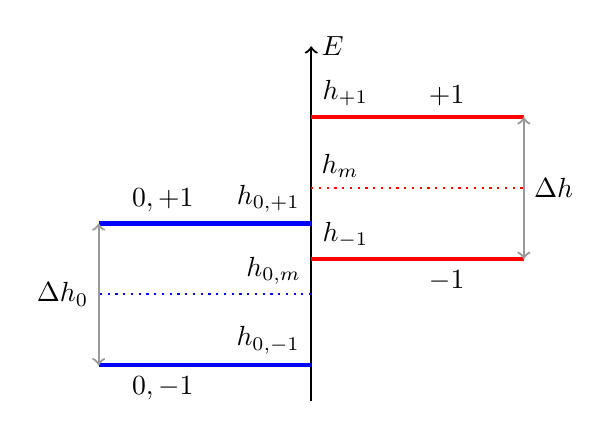
\begin{tikzpicture}[scale=0.9]
        \draw[->,black,thick] (0,-1) -- (0,4)node[anchor=west]{$E$};
        \draw[blue,ultra thick] (0,-.5)node[anchor=south east,black]{$h_{0,-1}$} --node[anchor=north east ,black]{$\ket{0,-1}$} (-3,-.5);
        \draw[blue,ultra thick] (0,1.5)node[anchor=south east,black]{$h_{0,+1}$}  --node[anchor=south east,black]{$\ket{0,+1}$} (-3,1.5);
        \draw[blue, thick,dotted] (0,.5)node[anchor= south east,black]{$h_{0,m}$}  -- (-3,.5);
        \draw[<->,black!40,thick] (-3,-.5) --node[anchor=east,black]{$\Delta h_{0}$} (-3,1.5);

        \draw[red,ultra thick] (0,1)node[anchor=south west,black]{$h_{-1}$} --node[anchor=north west,black]{$\ket{-1}$} (3,1);
        \draw[red,ultra thick] (0,3)node[anchor=south west,black]{$h_{+1}$}  --node[anchor=south west,black]{$\ket{+1}$} (3,3);
        \draw[red, thick,dotted] (0,2)node[anchor=south west,black]{$h_{m}$}  -- (3,2);
        \draw[<->,black!40,thick] (3,1) --node[anchor=west,black]{$\Delta h$} (3,3);
    \end{tikzpicture}
\end{figure}

Le espressioni ottenute possono essere approssimate nel caso in cui la perturbazione sia piccola, ossia se vale la seguente condizione:
\begin{equation*}
    |\underline{w}|\ll h_{0,m},\ \Delta h_0.
\end{equation*}
In questo caso valgono le seguenti approssimazioni\footnote{Si ricorda l'approssimazione in serie di Taylor $\sqrt{1+x}=1+x/2-x^2/8+O(x^3)$.}:
\begin{flalign*}
    \bigg|\frac{\Delta h_{0}}{2}\underline{e}_0+\underline{w}\bigg|&=\sqrt{\bigg(\frac{\Delta h_{0}}{2}\bigg)^2+\Delta h_{0}w_0+|\underline{w}|^2}=\frac{\Delta h_0}{2}\sqrt{1+\bigg[\frac{4w_0}{\Delta h_0}+\bigg(\frac{2|\underline{w}|}{\Delta h_{0}}\bigg)^2\bigg]}\\&=\frac{\Delta h_0}{2}\bigg[1+\frac{1}{2}\bigg[\frac{4w_0}{\Delta h_0}+\bigg(\frac{2|\underline{w}|}{\Delta h_{0}}\bigg)^2\bigg]-\frac{1}{8}\bigg[\frac{4w_0}{\Delta h_0}+\bigg(\frac{2|\underline{w}|}{\Delta h_{0}}\bigg)^2\bigg]^2+O\bigg(\frac{|\underline{w}|}{\Delta h_{0}}\bigg)^3\bigg]\\&=\frac{\Delta h_0}{2}\bigg[1+\frac{2w_0}{\Delta h_0}+2\bigg(\frac{|\underline{w}|}{\Delta h_{0}}\bigg)^2-2\bigg(\frac{w_0}{\Delta h_{0}}\bigg)^2+O\bigg(\frac{|\underline{w}|}{\Delta h_{0}}\bigg)^3\bigg]\\&=\frac{\Delta h_0}{2}+w_0+\frac{|\underline{w}|^2-w_0^2}{\Delta h_{0}}+O\bigg(\frac{|\underline{w}|^3}{\Delta h_{0}^2}\bigg)\\&=\frac{\Delta h_0}{2}+w_0+\frac{w_{+1}w_{-1}}{\Delta h_{0}}+O\bigg(\frac{|\underline{w}|^3}{\Delta h_{0}^2}\bigg),\\
    \Longrightarrow\qquad &\boxed{h_{\pm1}=h_{0,m}+w_m\pm\bigg[\frac{\Delta h_0}{2}+w_0+\frac{w_{+1}w_{-1}}{\Delta h_{0}}\bigg]+O\bigg(\frac{|\underline{w}|^3}{\Delta h_{0}^2}\bigg)}\ .
\end{flalign*}
Con conti analoghi si ottiene: l'approssimazione degli autostati
\begin{equation*}
    \boxed{\ket{\pm1}=\ket{0,\pm1}\pm\ket{0,\pm1}\frac{w_{\pm 1}}{\Delta h_0}+O\bigg(\frac{|\underline{w}|^2}{\Delta h_{0}^2}\bigg)}\,
\end{equation*}
l'approssimazione della differenza di energia dei due livelli:
\begin{equation*}
    \boxed{\Delta h=\Delta h_0+2w_0+2\frac{w_{+1}w_{-1}}{\Delta h_{0}}+O\bigg(\frac{|\underline{w}|^3}{\Delta h_{0}^2}\bigg)}\ .
\end{equation*}